\begin{enumerate}
\item \begin{enumerate}
\item On dérive les deux termes de $g$, l'un des deux étant un produit.

On rappelle les dérivées connues : $\cos'=-\sin$ et $\sin'=\cos$.
\[
\forall x\in [0~;~2\pi],\quad g'(x)=1\times \cos(x)+x\times \left(-\sin(x)\right)-\cos(x)=-x\sin(x).
\]

\item Commençons par calculer les images de 0, $\pi$ et $2\pi$. On connaît les valeurs particulières des fonctions sinus et cosinus.
\begin{itemize}
\item $g(0)=0\times \cos(0)-\sin(0)=0\times 1-0=0$;
\item $g(\pi)=\pi\times \cos(\pi)-\sin(\pi)=\pi\times(-1)-0=-\pi$;
\item $g(2\pi)=2\pi\times \cos(2\pi)-\sin(2\pi)=2\pi\times 1-0=2\pi$.
\end{itemize}
Les trois images sont donc validées.

Étudions maintenant les variations de $g$.
\begin{itemize}
\item sur $[0~;~2\pi]$, $-x$ est négatif, et même strictement négatif sur $]0~;~2\pi]$;
\item sur $[0~;~\pi]$, $\sin(x)$ est positif, et même strictement positif sur $]0~;~\pi[$ (c'est la moitié du cercle trigonométrique qui est au dessus de l'axe des abscisses, donc les sinus sont positifs);
\item sur $[\pi~;~2\pi]$, $\sin(x)$ est négatif, et même strictement négatif sur $]\pi~;~2\pi[$ (c'est la moitié du cercle trigonométrique qui est en-dessous de l'axe des abscisses, donc les sinus sont négatifs).
\end{itemize}
On peut résumer cela avec un tableau de signes. Quand la dérivée est à valeurs négatives, la fonction est strictement décroissante (car la dérivée ne s'annule que ponctuellement), et quand la dérivée est à valeurs positives, la fonction est strictement croissante.

On a donc :

\begin{center}
	\begin{tikzpicture}
		\tkzTabInit[
		lgt=3.6,
		espcl=2.4,
		deltacl=0.6
		]
		{
			$x$ / 0.9,
			signe de $-x$ / 0.9,
			signe de $\sin(x)$ / 0.9,
			signe de $g'(x)$ / 0.9,
			variations de $g$ / 1.8
		}
		{$0$, $\pi$, $2\pi$}
		
		\tkzTabLine{z, -, -, -, -}
		\tkzTabLine{z, +, z, -, z}
		\tkzTabLine{z, -, z, +, z}
		\tkzTabVar{+/$0$, -/$-\pi$, +/$2\pi$}
	\end{tikzpicture}
\end{center}

\item La fonction $g$ est continue (car dérivable) sur $[\pi~;~2\pi]$, sur cet intervalle, elle est strictement croissante.

De plus, 0 est une valeur intermédiaire entre $f(\pi)=-\pi$ et $f(2\pi)=2\pi$.

D'après le corollaire du théorème des valeurs intermédiaires, il existe donc une unique solution à l'équation $g(x)=0$ dans l'intervalle $[0~;~2\pi]$, solution que l'on note $\alpha$.

\item On peut étoffer le tableau de variations précédent avec $\alpha$


\begin{center}
	\begin{tikzpicture}
		\tkzTabInit[
		lgt=3.2,
		espcl=2.2,
		deltacl=0.6
		]
		{$x$/1, signe de $g(x)$/1}
		{$0$, $\alpha$, $2\pi$}
		
		\tkzTabLine{z,-,z,+,}
	\end{tikzpicture}
\end{center}

Sur $[0~;~\alpha]$, la fonction $g$ est donc à valeurs négatives, puis sur $[\alpha~;~2\pi]$, elle est  à valeurs positives.


\end{enumerate}

\item \begin{enumerate}
\item On va utiliser la formule de dérivation d'un quotient :
\[
\forall x\in ]0~;~2\pi],\quad f'(x)=\dfrac{\cos(x)\times x-\sin(x)\times 1}{x^2}=\dfrac{x\cos(x)-\sin(x)}{x^2}=\dfrac{g(x)}{x^2}.
\]

\item La fonction $f'$ est le quotient de la fonction $g$ étudiée à la question 1. par la fonction carré.

On a donc :

\begin{center}
	\begin{tikzpicture}
		\tkzTabInit[
		lgt=3.2,
		espcl=2.2,
		deltacl=0.6
		]
		{$x$/1, signe de $g(x)$/1, signe de $x^2$/1, signe de $f'(x)$/1}
		{$0$, $\alpha$, $2\pi$}
		
		\tkzTabLine{z,-,z,+,}
		\tkzTabLine{z,+,+}
		\tkzTabLine{,-,z,+,}
	\end{tikzpicture}
\end{center}

\item On en déduit que la fonction $f$ est strictement décroissante sur l'intervalle $]0~;~\alpha]$ et strictement croissante sur $[\alpha~;~2\pi]$.

\item Pour tout réel $x$ non nul, le taux d'accroissement de la fonction sinus entre 0 et $x$ est :
\[
\dfrac{\sin(x)-\sin(0)}{x-0}=\dfrac{\sin(x)-0}{x}=\dfrac{\sin(x)}{x}=f(x).
\]
Comme la fonction sinus est dérivable en 0, ce taux d'accroissement admet donc une limite finie quand $x$ tend vers 0. Par définition du nombre dérivé, cette limite est le nombre dérivé de la fonction sinus en 0.

On a donc : $\displaystyle\lim_{x\to 0}f(x)=\sin'(0)=\cos(0)=1$.

$f$ tend vers 1 quand $x$ tend vers 0.
\end{enumerate}

\item On considère deux nombres réels $r$ et $s$ qui vérifient l'inégalité : $0<r<s<\pi$.

Comme $\alpha\in[\pi~;~2\pi]$, on en déduit que : $\pi\leq \alpha$.

Donc les réels $r$ et $s$ sont dans un intervalle où la fonction $f$ est strictement décroissante, et la fonction sinus à valeurs strictement positives :
\[
\begin{aligned}
0<r<s<\pi&\Longrightarrow f(r)>f(s)\\
&\Longrightarrow \dfrac{\sin(r)}{r}>\dfrac{\sin(s)}{s}\\
&\Longrightarrow \dfrac{\sin(r)}{r\times \sin(s)}>\dfrac1s \quad \text{car } s\in ]0~;~\pi[ \text{ donc } \sin(s)>0\\
&\Longrightarrow \dfrac{\sin(r)}{\sin(s)}>\dfrac rs \quad \text{car } r\in ]0~;~\pi[ \text{ donc } r>0.
\end{aligned}
\]
On a bien établi, pour $r$ et $s$ vérifiant $0<r<s<\pi$ :
\[
\dfrac rs<\dfrac{\sin(r)}{\sin(s)}.
\]
\end{enumerate}
